% !TEX root = ../metrics_hse_exams.tex

\subsection{Контрольная работа 1. ИП.}

\begin{enumerate}
\item (20 баллов) Была оценена регрессия вида

\[
Y_i = \beta_1 + \beta_2X_{i1} + \beta_3X_{i2} + \beta_4X_{i3} + \beta_5X_{i4} + \varepsilon_i.
\]

Результаты оценивания регрессии представлены в таблице ниже.

\begin{figure}[h]
	\begin{center}
				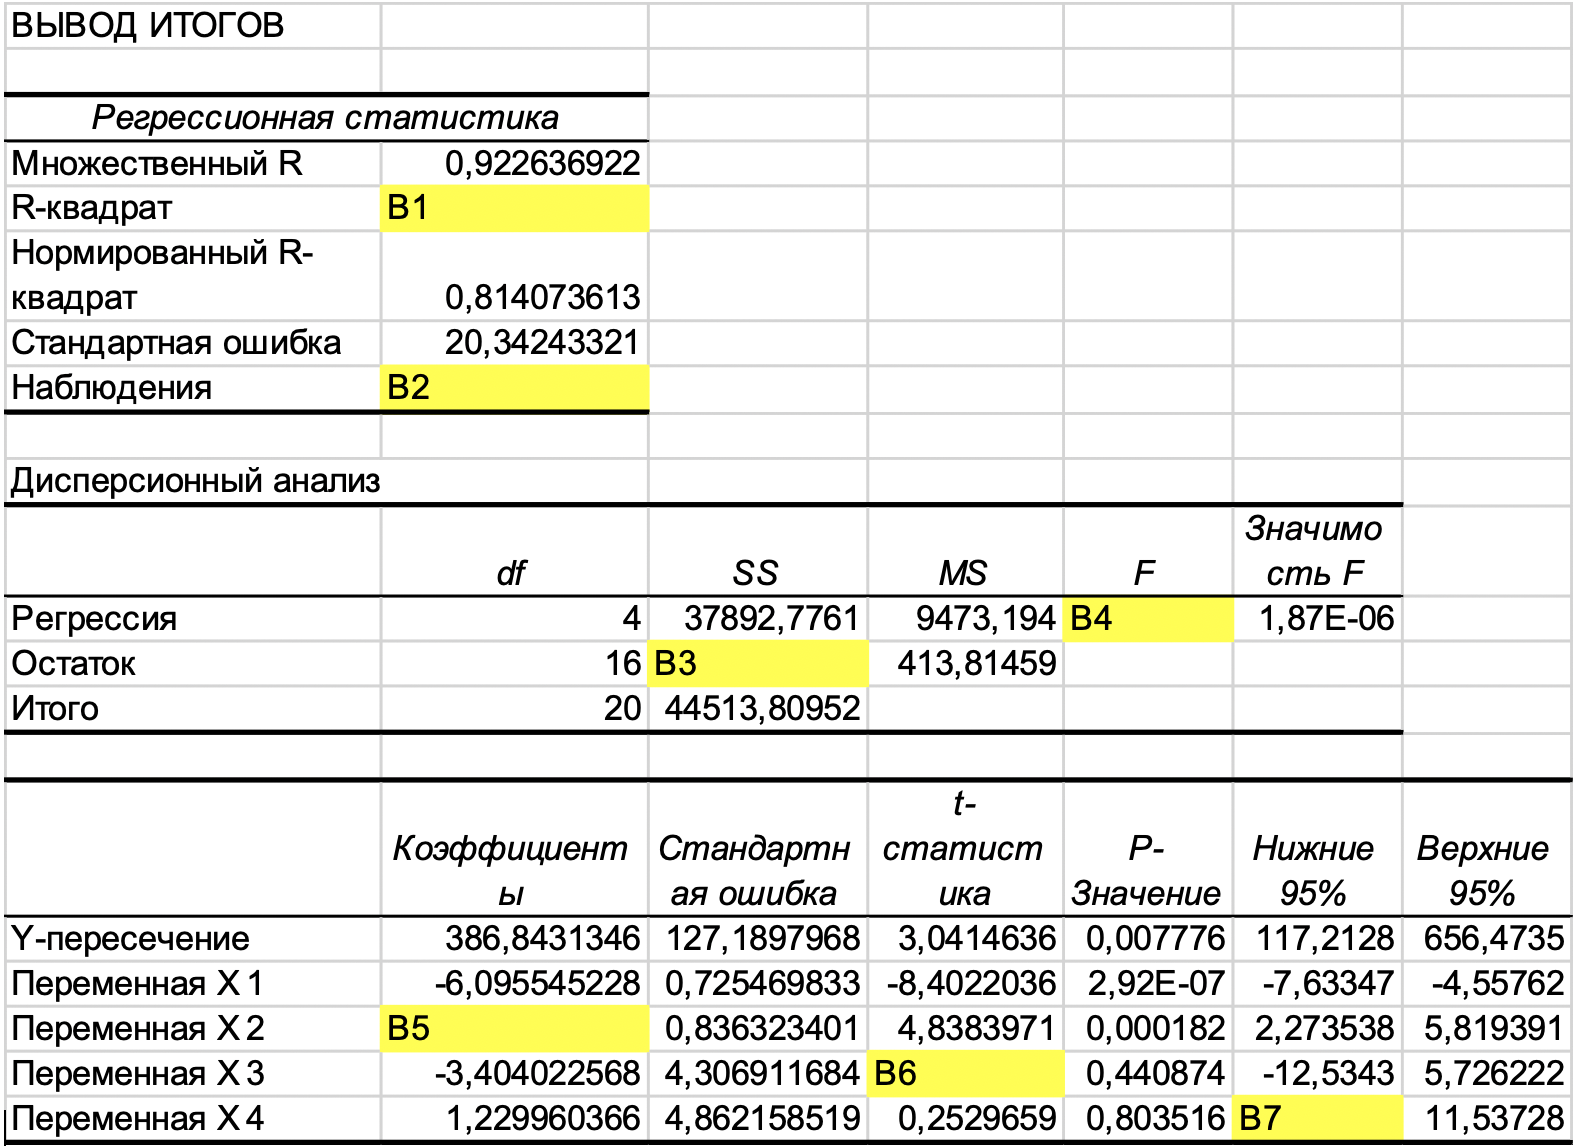
\includegraphics[scale=0.5]{figures/2022-2023_kr1.png}
	\end{center}
\end{figure}

\begin{enumerate}
\item (2 балла) Найдите значение B5.
\item (2 балла) Выпишите оцененное уравнение регрессии.
\item (2 балла) Найдите значение B1.
\item (2 балла) Найдите значение B2.
\item (2 балла) Найдите значение B3.
\item (2 балла) Найдите значение B4.
\item (2 балла) Найдите значение B6.
\item (2 балла) Найдите значение B7.
\item (4 балла) Сделайте вывод о значимости коэффициентов регрессии на уровне значимости 5\% и проинтерпретируйте полученные результаты.
\end{enumerate}

\item (20 баллов) Исследуется зависимость реального дохода на душу населения $y$ (в тыс.долл.) от процента рабочей силы, занятой в сельском хозяйстве, $x_1$ и среднего уровня образования населения в возрасте после 25 лет $x_2$ (число лет, проведенных в учебных заведениях) для 5 развитых стран в 2001 году. По имеющимся данным была оценена следующая модель регрессии:

\[
y_i = \beta_1 + \beta_2x_{i1} + \beta_3x_{i2} + \varepsilon_i.
\]

При этом известно, что

\[
X' X =  \begin{pmatrix}
5 & 3 & 1 \\
3 & 3 & 1 \\
1 & 1 & 1 \\
\end{pmatrix}, \quad (X' X)^{-1} =  \begin{pmatrix}
0.5 & -0.5 & 0 \\
-0.5 & 1 & -0.5 \\
0 & -0.5 & 1.5 \\
\end{pmatrix}, 
\]
\[
X'y =\begin{pmatrix}
15 \\
11 \\
4 
\end{pmatrix}, e'e = 6.5.
\]

\begin{enumerate}
\item (3 балла) Найдите МНК-оценки для параметров модели регрессии.
\item (3 балла) Проинтерпретируйте результаты регрессии.
\item (3 балла) Определите $\widehat{\sigma}^2_{\varepsilon}$, $\widehat{\sigma}^2_{\hb_2}$ и $\widehat{\sigma}^2_{\hb_3}$.
\item (3 балла) Постройте 95\%-ый доверительный интервал для $\beta_2$.
\item (3 балла) Проверьте на 5\%-ом уровне значимости гипотезу о том, что $\beta_2 = 0$ и $\beta_3 = 0$.
\item (2 балла) Спрогнозируйте реальный доход на душу населения для страны, в которой процент рабочей силы, занятой в сельском хозяйстве, составляет 7\% и средний уровень образования населения в возрасте после 25 лет составляет 12 лет.
\item (3 балла) Постройте 95\%-ый доверителный интервал для прогноза из предыдущего пункта.
\end{enumerate}

\item (10 баллов) Рассмотрим следующую регрессионную модель зависимости логарифма заработной платы $\ln (W)$ от уровня образования $Edu$ и опыта работы $Exp$, $Exp^2$:
 
\[
\widehat{\ln (W)_i} = \hb_0 + \hb_1 Edu_i + \hb_2 Exp_i + \hb_3 Exp^2_i.
\]

Модель регрессии была отдельно оценена по выборкам из 20 мужчин и 20 женщин, и
были получены остаточные суммы квадратов $RSS_{male} = 49.4$ и $RSS_{female} = 44.1$ Остаточная сумма квадратов в регрессии, оцененной по объединенной выборке ($RSS_{pooled}$), равна 105.5. Протестируйте на 5\%-ом уровне значимости гипотезу об отсутствии дискриминации в оплате труда между мужчинами и женщинами.

\item (10 баллов) Рассмотрим оценку вида $\tilde\beta = (X'X+rD)^{-1}X'y$ для вектора коэффициентов регрессионного уравнения $y = X\beta + \varepsilon$, где $D$ – диагональная $k \times k$ матрица, состоящая из диагональных элементов матрицы $X'X$.

\begin{enumerate}
\item (5 баллов) Найдите математическое ожидание оценки $\tilde\beta$.
\item (5 баллов) Найдите матрицу ковариаций оценки $\tilde\beta$.
\end{enumerate}
\end{enumerate}

\subsection{Экзамен. ИП.}





\subsubsection*{Часть I}

\begin{enumerate}
\item Признаком мультиколлинеарности не служит:
    \begin{enumerate}
    \item значительные изменения в оценках коэффициентов регрессии при небольших изменениях в данных
	\item близкое к 0 значение коэффициента множественной детерминации
	\item близкие к 0 значения коэффициентов корреляции регрессоров
	\item нелогичные знаки у коэффициентов
	\item нет верных вариантов ответа
    \end{enumerate}
\item По данным для 23 фирм была оценена зависимость выпуска $Y$ от труда $L$ и капитала $K$ с помощью следующих моделей: $\ln Y_i = \beta_1 + \beta_2 \ln K_i + \beta_3 \ln L_i + \varepsilon_i$ и $\ln Y_i = \alpha_1 + \alpha_2 (\ln K_i + \ln L_i) + u_i$. Суммы квадратов остатков в этих моделях, $RSS_1$ и $RSS_2$, соответственно равны 5 и 10. Тогда F–статистика для проверки гипотезы о равенстве эластичностей по труду и по капиталу  равна
	\begin{enumerate}
	\item 20
	\item 8
	\item 12
	\item 4
	\item нет верного ответа
	\end{enumerate}
\item Если p–value t-статистики при проверке значимости коэффициента регрессии равно 0.071, то этот коэффициент незначим при уровне значимости $\alpha$:
	\begin{enumerate}
	\item 0.05
	\item 0.1
	\item любом, большем, чем 0.071
	\item 0.7
	\item не менее 0.9075
	\end{enumerate}
\item Необходимыми условиями теоремы Гаусса – Маркова не являются
	\begin{enumerate}
	\item наличие в матрице Х единичного столбца
	\item правильная спецификация модели  
	\item постоянной дисперсии случайной составляющей
	\item равенство 0 математических ожиданий всех случайных составляющих
	\item нет правильного ответа.
	\end{enumerate}
\item Гетероскедастичность нельзя устранить:
	\begin{enumerate}
	\item добавив наблюдений в выборку
	\item сделав поправку Уайта
	\item разделить все регрессоры на корень из 10
	\item изменив функциональную форму модели
	\item удалив один из регрессоров модели
\end{enumerate}
\item Зависимость расходов домохозяйств на продовольственные товары $Y$ от располагаемого дохода $X$ (обе переменные измеряются в тыс. руб.) имеет вид: $\ln Y_i = -1.8 + 0.3\ln X_i$ (все коэффициенты регрессии значимы). При увеличении дохода на 1\% расходы увеличатся на:
	\begin{enumerate}
	\item 0.03 единицы
	\item 30\%
	\item 3\%
	\item 0.3\%
	\item нет верного ответа
	\end{enumerate}
\item Если оценивается модель $Y_i = \beta_1 + \beta_2 X_{i2} + \beta_3 X_{i3} + u_i$, а истинной является модель $Y_i = \beta_1 + \beta_2 X_{i2} + u_i$, то оценка МНК параметра $\beta_2$ в оцениваемой модели будет:
	\begin{enumerate}
	\item смещенной
	\item нелинейной
	\item неэффективной
	\item BLUE
	\item нет верного ответа
	\end{enumerate}
\item Тест Харке-Бера  используется:
	\begin{enumerate}
	\item для выявления гетероскедастичности
	\item для выявления значимости коэффициентов
	\item для определения правильной спецификации модели 
	\item для выявления мультиколлинеарности
	\item нет верного ответа
	\end{enumerate}
\item Оцененная по данным США зависимость заработной платы ($Wage$) от стажа ($Exp)$, пола ($Male$) (фиктивная переменная, равная 1 для мужчин и 0 для женщин), наличия высшего образования ($Educ$) (фиктивная переменная, равная 1 при наличии высшего образования и 0 иначе) и наличия детей в семье ($Children$) (фиктивная переменная, равная 1 при наличии детей в семье и 0 иначе) дала следующие результаты:
 \[
 \widehat{Wage}_i = 1.7 + 5.4 \cdot Exp_i + 0.5 \cdot Male_i + 2.3 \cdot Educ_i - 1.4 \cdot Children_i.
 \]
В этом случае заработная плата мужчины с высшим образованием, 5 годами стажа и двумя детьми будет равна:
	\begin{enumerate}
	\item 28.7
	\item 28.2
	\item 29.6
	\item 27.3
	\item 30.1
	\end{enumerate}
\item Сравнение линейной и полулогарифмической модели проводится с помощью теста:
	\begin{enumerate}
	\item Чоу
	\item Рамсея
	\item Бокса-Кокса
	\item VIF
	\item Глейзера
	\end{enumerate}

\end{enumerate}
\subsubsection*{Часть II}

Исследователь собрал следующие данные по 209 компаниям:

\begin{tabular}{cl}
\toprule
Переменная &	Описание переменной \\
\midrule
salary & Заработная плата топ-менеджера, тыс. долл \\
sales & Объем продаж, тыс. долл \\
lsalary & Логарифм заработной платы топ-менеджера \\
lsales & Логарифм объема продаж \\
pcsalary & Изменение заработной платы за год,  \\
roe & Отдача на собственный капитал компании,   \\
pcroe & Изменение отдачи на собственный капитал за год,  \\
ros & Изменение в цене акций компании за год, \\
indus & Dummy-переменная, принимающая 1 для промышленный компаний, \\
& 0 иначе. \\
finance & Dummy-переменная, принимающая 1 для компаний \\
& финансового сектора, 0 иначе. \\
consprod & Dummy-переменная, принимающая 1 для компаний, \\
& производящих потребительские товары, 0 иначе. \\
transport & Dummy-переменная, принимающая 1 для компаний, \\
& оказывающих транспортные услуги, 0 иначе. \\
\bottomrule
\end{tabular}


Основной целью исследователя была оценка следующей модели для объяснения вариации в заработной плате топ-менеджеров:

\[
lsalary_i= \beta_0 + \beta_1 \cdot lsales_i + \beta_2 \cdot pcsalary_i + 
\beta_3 \cdot roe_i +\beta_4 \cdot pcroe_i + \beta_5*ros + \varepsilon_i
\]

\begin{enumerate}
    \item (2 балла) Проинтепретируйте результаты оценивания регрессии (1). Какие факторы оказались значимы и на каком уровне значимости? Дайте количественную интерпретацию. Как бы Вы проинтерпретировали коэффициент при перекрестной переменной $pcsalary \cdot finance$ при наличии также переменной $finance$ в модели?
    \item (2 балла) Есть ли мультиколлинеарность в регрессии (1)? Ответьте на вопрос, используя различные критерии.
    \item (2 балла) Есть ли гетероскедастичность в модели (1)? Выпишите нулевую и альтернативную гипотезы теста.
    \item (2 балла) Есть ли ошибки спецификации в модели (1)? Выпишите нулевую и альтернативную гипотезы теста.
    \item (2 балла) Рассчитайте эластичность зависимой переменной по объемам продаж в точке средних значений.
    \item (2 балла) Проверьте совместную значимость всех дополнительных факторов в модели (2) по сравнению с моделью (1). Выпишите нулевую и альтернативную гипотезы теста.
    \item (2 балла) Проинтерпретируйте результаты оценки коэффициентов при дополнительных факторах в модели (2).
    \item (2 балла) Есть ли различия в моделях для финансовых и нефинансовых секторов (регрессии 3 и 4)? Выпишите нулевую и альтернативную гипотезы теста.
\end{enumerate}

Описательные статистики переменных 

\begin{tabular}{lrrrrr}
\toprule
Variable & N & Mean	& SD & Min & Max \\
\midrule
salary & 209 & 1281.12 & 1372.345 & 223 & 14822 \\
sales & 209 & 6923.793 & 10633.27 & 175.2 & 97649.9 \\
lsalary & 209 & 6.950386 & 0.566371 & 5.40 & 9.60 \\
lsales & 209 & 8.2922 & 1.013161 & 5.165 & 11.489 \\
pcsalary & 209 & 13.2823 & 32.63392 & -61 & 212 \\
roe & 209 & 17.18421 & 8.518509 & 0.5 & 56.3 \\
pcroe & 209 & 10.80048 & 97.2194 & -98.9 & 977 \\
ros & 209 & 61.80383 & 68.17705 & -58 & 418 \\
indus & 209 & 0.320574 & 0.467818 & 0 & 1 \\
finance & 209 & 0.220096 & 0.415306 & 0 & 1 \\
consprod & 209 & 0.287081 & 0.453486 & 0 & 1 \\
\bottomrule
\end{tabular}

Корреляционная матрица

\begin{tabular}{ccc ccc ccc c}
\toprule
& lsalary & lsales & pcsalary	& roe & pcroe & ros & indus	& finance & consprod \\
\midrule
lsalary	& 1 &&&& &&&& \\
lsales	& 0.4591 & 1 &&& &&&& \\	
pcsalary & 0.0438 & -0.0652 & 1 &&& &&& \\
roe	& 0.2085 & -0.1226 & 0.0873 & 1 &&&&& \\
pcroe & 0.1077 & 0.0233	& 0.208	& 0.0042 & 1 &&&& \\
ros & -0.0746 & -0.3503	& 0.1378 & 0.2749 &	0.1289 & 1 &&& \\
indus & -0.0161	& 0.0603 & 0.0044 & 0.0135 & -0.0296 & -0.2095 & 1 && \\	
finance & 0.1008 & 0.039 & -0.0908 & -0.1785 & 0.0917 & -0.108 & -0.3649 & 1 & \\
consprod & 0.2203 & -0.0191 & 0.052 & 0.4085 & -0.0157  & 0.3478 & -0.4359 & -0.3371 & 1 \\
\bottomrule
\end{tabular}

\subsubsection*{Часть III}

\begin{enumerate}
    \item (6 баллов). В некотором аналитическом центре работает $n$ аналитиков. Их производительность труда описывается следующей функцией:
\[
y_i = \beta_1 + \beta_2 \cdot MSU_i+\beta_3 \cdot HSE_i+\varepsilon_i, \quad i=1,2, \ldots, n.
\]
Здесь $y_i$ — производительность труда $i$-го аналитика; $MSU_i$ — переменная, равная единице, если $i$-й аналитик является выпускником магистратуры МГУ, и равная нулю в противном случае; $HSE_i$ — переменная, равная единице, если $i$-й аналитик является выпускником магистратуры НИУ ВШЭ, и равная нулю в противном случае. Все аналитики в компании заканчивали либо только магистратуру МГУ, либо только магистратуру НИУ ВШЭ, либо не заканчивали магистратуру вовсе. 

Случайные ошибки $\varepsilon_i$ удовлетворяют всем предпосылкам классической линейной модели множественной регрессии. Параметры $\beta_2$ и $\beta_3$ — положительные.
Прочие факторы, кроме указанных в уравнении, не влияют на производительность труда аналитиков.
Экономист ААА готовит исследование «Магистерские программы МГУ и производительность труда». На основе данных про всех аналитиков компании при помощи МНК он оценивает параметры модели парной регрессии $\hy_i = \hb_1 + \hb_2 MSU_i$, игнорируя вторую бинарную переменную.
\begin{enumerate}
    \item (3 балла) Пусть производительность аналитиков из МГУ и ВШЭ различна: $\beta_2 > \beta_3$. Будет ли $\hb_2$ несмещенной оценкой параметра $\beta_2$? Если да, то почему? Если нет, то будет ли она завышена или занижена?
Формально обоснуйте свой ответ. Вы можете использовать готовые формулы для МНК-оценок коэффициентов, но всё остальное следует подробно вывести.
\item (3 балла) Изменится ли ваш ответ на вопросы предыдущего пункта, если в действительности производительность аналитиков из МГУ и ВШЭ совпадает $(\beta_2 = \beta_3)$?
\end{enumerate}

    \item (5 баллов) В своей статье Д. Асемоглу, С. Джонсон и Дж. Робинсон анализируют
    воздействие качества экономических институтов на экономическое развитие,
    если точнее, речь идет о защите прав собственности. 
    В качестве объясняющей переменной авторы используют индекс, характеризующий защиту прав собственности в данной стране. 
    Индекс рассчитывается на основе ряда переменных и нормирован таким образом, что большее значение индекса означает более высокий уровень защиты прав собственности. 
    Зависимая переменная — ВВП на душу населения в данной стране (в долларах).
    
Поясните, с какими источниками эндогенности регрессора авторы скорее всего должны были столкнуться в своей статье. Какое решение этой проблемы в модели Вы можете предложить?

\textit{Источник: Acemoglu D., Johnson S., Robinson J. A. 2001. The Colonial Origins of Comparative Development: An Empirical Investigation, American Economic Review. Vol. 91(5).}

    \item Рассмотрим модель регрессии 
    \[
    y_i = \alpha x_i + \varepsilon_i,
    \]
где $\varepsilon_i$ – независимые случайные величины с нулевым математическим ожиданием и условной дисперсией $\Var(\varepsilon_i \mid x_i) = \sigma^2_0 \cdot x^{0.5}_i$. 
В вашем распоряжении имеется выборка из $n$ наблюдений $(x_i, y_i), x_i > 0, i = 1, \ldots, n$. 
Используя взвешенный метод наименьших квадратов, найдите эффективную оценку параметра $\alpha$. 
Задайте оценку $\hat\alpha$ как функцию от исходных данных $(x_i, y_i),  i = 1, \ldots, n$.

    \item Рассмотрим модель:
\[
\ln y_t = \beta_1 + \beta_2 \ln x_t + \beta_3 d_t \ln x_t + \varepsilon_t,
\]
где $y_t$ — величина спроса $i$-го индивида на товар $N$ в кг; $x_t$ – доход индивида, тыс. руб.; $d_t$ – бинарная переменная, равная единице для женщин и нулю для мужчин.
Оценка параметров модели при помощи МНК на основе данных о 1000 индивидов дала следующие результаты:
\[
\widehat{\ln y_t} = \underset{(0.12)}{1.22} + \underset{(1.00)}{10.00} \ln x_t - \underset{(2.00)}{11.00}d_t \ln x_t .
\]

Известно, что $\hCov(\hb_2, \hb_3)=2.0$ и $\hCorr(\ln x_t, d_t \ln x_t)=0.04$.

\begin{enumerate}
\item  (3 балла) Влияет ли изменение дохода на потребление товара N женщинами (сформулируйте и проверьте соответствующую гипотезу при уровне значимости 5\%)? Если да, то укажите, на сколько килограммов (или процентов) и в каком направлении меняется спрос на товар $N$ в результате увеличения дохода женщины на 1\%?
\item (2 балла) Влияет ли изменение дохода на потребление товара $N$ мужчинами (сформулируйте и проверьте соответствующую гипотезу при уровне значимости 5\%)? Если да, то укажите, на сколько килограммов (или процентов) и в каком направлении меняется спрос на товар N в результате увеличения дохода мужчины на 1\%?
\item (2 балла) Есть ли в рассматриваемой модели существенная мультиколлинеарность? Обоснуйте свой ответ, вычислив соответствующий коэффициент VIF.
\end{enumerate}




\end{enumerate}
